%% Version 4.3.2, 25 August 2014
%
%%%%%%%%%%%%%%%%%%%%%%%%%%%%%%%%%%%%%%%%%%%%%%%%%%%%%%%%%%%%%%%%%%%%%%
% Template.tex --  LaTeX-based template for submissions to the 
% American Meteorological Society
%
% Template developed by Amy Hendrickson, 2013, TeXnology Inc., 
% amyh@texnology.com, http://www.texnology.com
% following earlier work by Brian Papa, American Meteorological Society
%
% Email questions to latex@ametsoc.org.
%
%%%%%%%%%%%%%%%%%%%%%%%%%%%%%%%%%%%%%%%%%%%%%%%%%%%%%%%%%%%%%%%%%%%%%
% PREAMBLE
%%%%%%%%%%%%%%%%%%%%%%%%%%%%%%%%%%%%%%%%%%%%%%%%%%%%%%%%%%%%%%%%%%%%%

%% Start with one of the following:
% DOUBLE-SPACED VERSION FOR SUBMISSION TO THE AMS
\documentclass{ametsoc}

% TWO-COLUMN JOURNAL PAGE LAYOUT---FOR AUTHOR USE ONLY
% \documentclass[twocol]{ametsoc}

%%%%%%%%%%%%%%%%%%%%%%%%%%%%%%%%
%%% To be entered only if twocol option is used

\journal{jcli}

%  Please choose a journal abbreviation to use above from the following list:
% 
%   jamc     (Journal of Applied Meteorology and Climatology)
%   jtech     (Journal of Atmospheric and Oceanic Technology)
%   jhm      (Journal of Hydrometeorology)
%   jpo     (Journal of Physical Oceanography)
%   jas      (Journal of Atmospheric Sciences)	
%   jcli      (Journal of Climate)
%   mwr      (Monthly Weather Review)
%   wcas      (Weather, Climate, and Society)
%   waf       (Weather and Forecasting)
%   bams (Bulletin of the American Meteorological Society)
%   ei    (Earth Interactions)

%%%%%%%%%%%%%%%%%%%%%%%%%%%%%%%%
%Citations should be of the form ``author year''  not ``author, year''
\bibpunct{(}{)}{;}{a}{}{,}
\usepackage[super]{nth} %adds superscripts for things like 20th

%%%%%%%%%%%%%%%%%%%%%%%%%%%%%%%%

%%% To be entered by author:

%% May use \\ to break lines in title:

\title{A 57-year catalog of frontal rainfall in China using the Rainband Detection Algorithm (RDA). Part II: Interannual Variations}

%%% Enter authors' names, as you see in this example:
%%% Use \correspondingauthor{} and \thanks{Current Affiliation:...}
%%% immediately following the appropriate author.
%%%
%%% Note that the \correspondingauthor{} command is NECESSARY.
%%% The \thanks{} commands are OPTIONAL.

    %\authors{Author One\correspondingauthor{Author One, 
    % American Meteorological Society, 
    % 45 Beacon St., Boston, MA 02108.}
% and Author Two\thanks{Current affiliation: American Meteorological Society, 
    % 45 Beacon St., Boston, MA 02108.}}

\authors{Jesse A. Day\correspondingauthor{Jesse Day, University of California, Department of Earth and Planetary Science, College of Letters and Science, 307 McCone Hall, Berkeley, CA 94720.}, Inez Y. Fung and John C. H. Chiang}

\affiliation{Department of Earth and Planetary Science, University of California Berkeley, Berkeley, California}

%% Follow this form:
    %\email{latex@ametsoc.org}

\email{jessed@berkeley.edu}

%% If appropriate, add additional authors, different affiliations:
    %\extraauthor{Extra Author}
    %\extraaffil{Affiliation, City, State/Province, Country}

%\extraauthor{}
%\extraaffil{}

%% May repeat for a additional authors/affiliations:

%\extraauthor{}
%\extraaffil{}

%%%%%%%%%%%%%%%%%%%%%%%%%%%%%%%%%%%%%%%%%%%%%%%%%%%%%%%%%%%%%%%%%%%%%
% ABSTRACT
%
% Enter your abstract here
% Abstracts should not exceed 250 words in length!
%
% For BAMS authors only: If your article requires a Capsule Summary, please place the capsule text at the end of your abstract
% and identify it as the capsule. Example: This is the end of the abstract. (Capsule Summary) This is the capsule summary. 

\abstract{In the second stage of our study, we investigate how interannual variations in China rainfall are manifested in the RDA catalog, and also attempt to pin down the particular changes in banded rainfall that caused the ``South Flood-North Drought'' pattern of late \nth{20}-century rainfall change in China. Two robust changes occurred during 1980-2007 relative to 1951-1979: 1) A decrease in the frequency of frontal rainbands during the Pre-Meiyu period (May), and 2) a southward shift in the latitude of Post-Meiyu rainbands (mid-July to September. This latter change is predominantly responsible for the changes in yearly mean rainfall described as the South Flood-North Drought. The RDA method reveals alterations in rainband behavior that are not captured by other simpler metrics of China rainfall.}

% In addition, a previously reported shifted in June-July rainfall between 1994-2007 and 1979-1993 resulted from a change in intensity of frontal rainfall events, even though their frequency remained constant

%By studying historical rainfall change, we begin to address the critical question of whether the South Flood-North Drought will persist under \nth{21}-century global warming.

\begin{document}

%% Necessary!
\maketitle


%%%%%%%%%%%%%%%%%%%%%%%%%%%%%%%%%%%%%%%%%%%%%%%%%%%%%%%%%%%%%%%%%%%%%
% MAIN BODY OF PAPER
%%%%%%%%%%%%%%%%%%%%%%%%%%%%%%%%%%%%%%%%%%%%%%%%%%%%%%%%%%%%%%%%%%%%%
%

%% In all cases, if there is only one entry of this type within
%% the higher level heading, use the star form: 
%%
% \section{Section title}
% \subsection*{subsection}
% text...
% \section{Section title}

%vs

% \section{Section title}
% \subsection{subsection one}
% text...
% \subsection{subsection two}
% \section{Section title}

%%%
% \section{First primary heading}

% \subsection{First secondary heading}

% \subsubsection{First tertiary heading}

% \paragraph{First quaternary heading}

\section{Introduction}

	A growing volume of evidence suggests a shift in rainfall over China beginning in the late 1970s, featuring a ``South Flood-North Drought'' pattern shown in Figure~\ref{fig:f31} \citep{Hu1997,Gong2002,Nigam2013}.  A permanent change would have major humanitarian impacts on densely-populated eastern China, where a sizable fraction of the population depends on agriculture for subsistence. Northern China already suffers from substantial depletion of freshwater resources along with increasing demand \citep{Currell2012,Gleeson2012}. The Chinese government has embarked on a project to reroute water from the Yangtze River to northern China, the South-North Water Transfer Project (\textit{nanshui beidiao gongcheng}), which is expected to become the most expensive hydraulic engineering project ever undertaken and will entail massive human and environmental impact \citep{Magee2011}. Under such circumstances, it is vital to understand whether this pattern will strengthen under global warming, or represents only a temporary deviation from the mean. 
	
	We use the RDA catalog to find the late \nth{20}-century changes in rainband statistics that have caused the South Flood-North Drought. As demonstrated in Part 1, banded rainfall contributes a large fraction of yearly rainfall totals in China. Therefore, the South Flood-North Drought may have been produced by changes in rainband progression such as a shift in latitude, a change in intensity, or an earlier or delayed northward migration. In turn, such a characterization may elucidate the large-scale dynamics responsible for the change. Since rainbands are produced by frontal atmospheric conditions, late \nth{20}-century changes in rainband attributes may reflect corresponding changes in East Asian monsoon dynamics, and may ultimately reflect the influence of \nth{20}-century warming. 

\section{Methods}

\subsection{Temporal Autocorrelation}

	Fronts and rainbands tend to persist for several days. Therefore, rainfall amounts and front attributes on successive days are not fully independent observations, which reduces the effective number of degrees of freedom of these time series. This temporal autocorrelation must be accounted for in calculations of statistical significance such as estimating the $p$-value of a change in rainband frequency between two time periods. In this particular case, we use the analytic formula for a Bernoulli process (applicable for any time series where observations are binary) with effective number of degrees of freedom $n=\frac{N}{\tau}$ for number of days $N$ and decorrelation time $\tau$ given by

\begin{equation*}
\tau=1+2\sum_{k=1}^m \rho(k)
\end{equation*}

	where $\rho(k)$ is the autocorrelation function of rainband existence with lag $k$ \citep{VonStorch1999}. We calculate $\tau$ using a maximum lag of $m=10$ days. The yearly mean decorrelation timescale of rainband frequency is found to be $\tau = 1.81$ after removing the seasonal cycle. This value is used to calculate significance of changes in Figure 3b. The standard deviation and $p$-values of rainband frequency changes in Tables~\ref{tab:t35} and~\ref{tab:t37} use seasonal values of $\tau$ calculated in \ref{tab:t34}. Similarly, Table~\ref{tab:t311} shows the $\tau$ of alternative metrics of China rainfall, which is then used to calculate the significance of decadal changes in Table~\ref{tab:t312}. $\tau$ is also used to select block length for moving blocks bootstrap tests, as described below.

%% BOOTSTRAPPING
\subsection{Significance of Changes: Bootstrapping Algorithms}

	Observations of rainband latitude and intensity during a given time period obey unknown distributions. Therefore, we require non-parametric tests to estimate the standard deviation of their mean and the significance of changes in mean. We employ bootstrapping with and without replacement (the latter also known as a permutation test), well-established techniques that estimate quantities of interest by constructing synthetic distributions with random sampling of original data \citep{Good2005}. We use bootstrapping with replacement to calculate the standard deviation of means (Tables~\ref{tab:t34},~\ref{tab:t36} and~\ref{tab:t38}). We focus on changes in front attributes between 1951-1979 and 1980-2007 (Tables~\ref{tab:t35} and~\ref{tab:t36}), and also repeat our methodology for 1979-1993 versus 1994-2007 (Tables~\ref{tab:t37} and~\ref{tab:t38}). $p$-values listed are from permutation testing with 10,000 iterations; the results of bootstrapping with and without replacement are very similar.
	
	The bootstrap must be adapted for time series featuring temporal autocorrelation. In such time series, a single anomalous weather event will persist over several days, and a bootstrap method will tend to exaggerate the significance of differences between the two original distributions. To avoid this scenario, we use a \textit{moving blocks bootstrap} test, described for instance in \citet{Singh2014}. This technique is identical to bootstrapping with replacement except that samples are drawn in continuous blocks of length $n$ that preserve the time structure of the original data set. Block length is chosen based on decorrelation time scale $\tau$. The autocorrelation of daily rainfall in China is $\tau =\mytilde 3$ days, and therefore the significance estimates in Figure~\ref{fig:hov}a use a moving blocks bootstrap with block length of 3 days and 1000 iterations. The calculation of significance of change in alternative China rainfall statistics $M_1-M_6$ (Table~\ref{tab:t312}) uses the $\tau$ of each statistic in each season (Table~\ref{tab:t311}) rounded to the nearest integer as block length. In general, a choice of block lengths between 2 and 5 days leads to similar results. Our MATLAB code for the permutation test and the moving blocks bootstrap is included in the appendix.
	
	The moving blocks bootstrap cannot be used for time series with gaps. Therefore, we use a permutation test to estimate the significance of changes in mean latitude and intensity of rainbands between time periods (Tables~\ref{tab:t36} and~\ref{tab:t38}). These latter results are verified with Anderson-Darling and Kolmogorov-Smirnov tests, two methods which estimate the significance of shifts in distribution between two sample. These tests are described below.

\subsection{Significance of Changes in Distribution}

In addition to gauging the significance of changes in mean, we can also test the probability that two samples were drawn from the same distribution. The Kolmogorov-Smirnov and Anderson-Darling tests each define a test statistic based on the largest difference between the observed probability distribution of two samples. Similar to a $t$-test, the value of this test statistic can be translated into a $p$-value. We first define the \textit{empirical distribution function} $F_1(x)$ and $F_2(x)$ of each sample. All $n$ observations in each sample are ordered as $\left\{X_1 < ... < X_n\right\}$, after which $F(x)$ is calculated as follows:

\begin{align}
	F(x) =& \frac{1}{n}\sum_{i=1}^n I_{[-\infty,x]} (X_i) \\
	I_{[-\infty,x]} =& 
	\begin{cases}
   		 1 & \text{if } X_i \leq x\\
    		0 & \text{otherwise} \\
    	\end{cases}
\end{align}

 The K-S test statistic $D$ is then defined as the maximal distance between the two empirical distribution functions:

\begin{equation}
	D=\max_{all\ x} |F_{1}(x)-F_{2}(x)|
\end{equation}

$D$ can then be inverted to derive a $p$-value. The Anderson-Darling (A-D) test statistic $A^2$ resembles $D$, but is formulated to be more sensitive to the tails of the distribution:

\begin{equation}
	A^2 = -n-S \,,
	\mathrm{where}
\end{equation}

\begin{equation}
	S=\sum_{i=1}^n \frac{2i-1}{n}\left[\ln(F(X_i)) + \ln\left(1-F(X_{n+1-i})\right)\right].
\end{equation}

$A^2$ can likewise be translated into a $p$-value. The K-S and A-D tests cannot be used if values are repeated within samples, because $D$ and $A^2$ are then undefined. We solve this problem by using bootstrap versions of these tests. Bootstrap K-S and A-D tests were performed using the programming language R with 10,000 iterations. The significance of changes in the distribution of rainband latitude and intensity are presented in Tables~\ref{tab:t313} and~\ref{tab:t314}. Both tests produce fairly similar results.

\section{Results}

\subsection{1980-2007 versus 1951-1979}

%% NEW PARAGRAPH - SIMPLY DESCRIBES THE YEARLY CUMULATIVE SOUTH FLOOD-NORTH DROUGHT
	The yearly mean change in rainfall rate between 1951-1979 and 1980-2007 over the region 100$^{\circ}$-142$^{\circ}$E and 20$^{\circ}$-48$^{\circ}$N is shown in Figure~\ref{fig:f31}. The South Flood-North Drought refers in particular to a meridional dipole of decadal rainfall change over eastern China (110$^{\circ}$-125$^{\circ}$E and 22$^{\circ}$-42$^{\circ}$N), where most of China's population resides. Pronounced local shifts are also visible in Taiwan, South Korea and parts of Japan. This work focuses on eastern China. Annual changes in northern China between 35$^{\circ}$-40$^{\circ}$N are significant at a 95\% confidence level, whereas changes in central and southern China are not. However, there are substantial changes in central and southern China rainfall during particular Meiyu stages, as shown in Figure~\ref{fig:changes}a and discussed below.
		
	We test whether the rainband catalog reflects the South Flood-North Drought by calculating changes in rainband frequency during 1980-2007 relative to 1951-1979 (shown as a Hovm\"oller diagram in Figure~\ref{fig:changes}b). We also calculate the significance of changes in rainband attributes during each of the five Meiyu stages (Tables~\ref{tab:t35} and~\ref{tab:t36}). During the Pre-Meiyu (days 121-160), the probability of observing a primary rainband has declined from $59.0\% \pm 2.0\%$ to $53.0\% \pm 2.1\%$ ($p=0.020$; Table~\ref{tab:t35}. Figure~\ref{fig:changes} shows matching decreases in front occurrence and rainfall over central China during this time period. The Pre-Meiyu decrease in rainfall was previously reported by \citet{Xin2006}, who linked it to decadal change in the North Atlantic Oscillation (NAO), and also by \citet{Wang2009}. We propose that diminished rainband occurrence has caused this decrease.
		
	In addition, a southward shift in mean rainband latitude has occurred during the Post-Meiyu (days 201-273, or July 20-Sep 30). We focus on rainbands north of 27$^{\circ}$N; rainbands occurring south of this latitude are produced by the westward-propagating remnants of tropical storms, and therefore dynamically unrelated to other storminess during Meiyu season \citep{Day2015}. Considering both primary and secondary rainbands north of 27$^{\circ}$N, mean latitude during 1951-1979 was $33.6^\circ \textrm{N} \pm .3^\circ$ versus $32.9^\circ \textrm{N} \pm .3^\circ$ during 1980-2007 ($p=.0003$; Table~\ref{tab:t36}). This shift remains significant if we do not restrict by front latitude ($p=.0048$). A Post-Meiyu rainfall increase in central China and decrease in northern China has also occurred, producing a South Flood-North Drought pattern (Figure~\ref{fig:changes}c). As a result, yearly rainfall has increased in central China even though Pre-Meiyu rainfall changes in that region are actually negative (Figure~\ref{fig:changes}a). Unlike \citet{Yu2010}, our catalog does not exhibit a \nth{20}-century decrease in the intensity of Yangtze River region frontal rainbands during July-August. A significant southward shift in rainband latitude is also found for the whole year ($p=.0032$, Table~\ref{tab:t36}), but this signal is dominated by the Post-Meiyu shift.
	
	%SHORT PARAGRAPHLET on the 1979-1993 v 1994-2007 jump.
\subsection{1979-1993 versus 1994-2007}
	
	We test this methodology also with the set of years 1979-1993 versus 1994-2007, when past authors have reported a shift in South China rainfall \citep{Kwon2007,Wu2010,Yim2013}. The most distinctive change between these two sets of years occurred during Meiyu season, during which rainband latitude shifted southward from $30.0^\circ \textrm{N} \pm .4^\circ$ to $28.9^\circ \textrm{N} \pm .4^\circ\ (p=.0002)$ and the \textit{intensity} of rainbands also jumped from $27.3 \pm 1.1$ mm day$^{-1}$ to $29.8 \pm 1.1$ mm day$^{-1}\ (p=.9994)$, leading to increased rainfall over central and southern China. \citet{Zou2015} also found that China experienced a more intense Meiyu during the 1990s, as well as generally more severe rainfall events. Unlike the comparison between 1951-1979 and 1980-2007, rainband \textit{frequency} remained unchanged. We infer that changes in frequency versus changes in intensity may signal the existence of two different types of external forcing, an idea further explored in the conclusion.
	
	%% ANDERSON-DARLING AND KOLMOGOROV-SMIRNOV TESTING 
\subsection{Significance of Changes in Distribution of Latitude and Intensity}

	As discussed in Section 3.5, a permutation test of changes in rainband latitude and intensity may exaggerate their significance. We use two independent techniques, a bootstrap Kolmogorov-Smirnov and bootstrap Anderson-Darling test, to verify the results in Table~\ref{tab:t34}. The results of comparing the years 1980-2007 to 1951-1979 is presented in Table~\ref{tab:t313}. Neither test captures the Pre-Meiyu decline in rainband frequency after 1979 since rainband latitude and intensity distributions remain similar. On the other hand, the Post-Meiyu southward shift in rainband latitude is found to be highly significant by both tests ($p<.001$). As before, no significant changes in rainband intensity are found between 1951-1979 and 1980-2007. This suggests that the estimates of significance from permutation testing are trustworthy.

	Also, a substantial southward shift in latitude and decrease in intensity of rainbands is found during Meiyu season between 1979-1993 and 1994-2007 ($p<.001$ for both changes; Table~\ref{tab:t314}). This further confirms that rainfall changes observed between 1979-1993 and 1994-2007 are fundamentally different from the South Flood-North Drought pattern of changes between 1951-1979 and 1980-2007.

\section{Conclusion}
	
	We are able to ascribe previously reported decadal rainfall change (the South Flood-North Drought) to modified rainband properties during particular rainfall stages. Two statistically significant occurred between the years 1951-1979 and 1980-2007: 

\begin{enumerate} 
\item A decrease in rainband frequency during the Pre-Meiyu ($p=.020$);
\item A southward shift in mean rainband latitude during the Post-Meiyu ($p=.0003$, permutation test; $p=.0001$, Anderson-Darling test). 
\end{enumerate}
	
	The first change led to a decrease in central China rainfall in May, while the second has been the principal contributor to the South Flood-North Drought trend in total yearly rainfall (Figure~\ref{fig:f31}). Furthermore, we find that rainfall changes during the Pre-Meiyu and Post-Meiyu in China are primarily due to changes in frontal rainfall, as opposed to a change in the contribution from local storms (Figure~\ref{fig:decadal_front}). These robust decadal changes in rainbands suggest the influence of large-scale climate change, which may have altered the synoptic conditions in the East Asian monsoon that produce frontal rainfall.
		
	It is essential to understand whether the South Flood-North Drought will persist under \nth{21}-century warming, or manifests an ephemeral decadal change. However, the CMIP5 (Climate Model Intercomparison Project) model suite contained in the Intergovernmental Panel on Climate Change's Fifth Assessment Report (IPCC AR5) does not even agree on the sign of future summer rainfall changes in East Asia \citep{Christensen2011}. Some studies attribute the South Flood-North Drought to natural variability \citep{Zhang1999,Xin2006,Lei2014}, but \citet{Zhou2009} claimed that the South Flood-North Drought was distinct from other patterns of \nth{20}-century variability. Since regional climate projection in Asia poses such a challenge, the most hopeful approach may be to link the South Flood-North Drought with other large-scale climate changes that can be more reliably modeled and projected into the future. \citet{Zhao2010} previously suggested that the South Flood-North Drought was associated with the late \nth{20}-century rise in global mean surface temperature. We suggest a link with observed changes in the seasonal cycle of the East Asian jet, which we will elaborate in future work.
		
%%1979-1993 v 1994-2007 - conclusion paragraph.
	We also investigated a change in China rainfall between 1979-1993 and 1994-2007 reported by other authors. We find a highly significant uptick in the \textit{intensity} of rainbands during Meiyu season ($p=.0006$) as well as a southward shift in their mean latitude ($p=.0002$). The resulting mid-summer rainfall increase over the Yangtze River basin has increased the risk of flooding \citep{Gemmer2008}. We suggest that a different mechanism explains this surge in frontal rainfall severity than explains the 1951-1979/1980-2007 changes, which are characterized by frequency changes. A potential culprit are the aerosols produced during the industrialization and urbanization of East China beginning in 1979 with Deng Xiaoping's Revolutionary Reform and Opening (\textit{gaige kaifang}). Recent research highlights the potentially substantial impact of aerosols on atmospheric temperature and cloud properties across Asia \citep{Menon2002,Fan2012,Streets2013}. We suggest that the intensification of frontal storms during Meiyu season from 1994 to 2007 is linked to the rise in aerosols, and that they may be further impacted by the anticipated decrease of anthropogenic aerosols in the \nth{21} century \citep{Westervelt2015}.
		
	Our study also shows that the whole of Taiwan has experienced a deficit in rainfall during the end of the twentieth century. In particular, the south and eastern coast on the east of the Central Mountain Range saw the largest decrease during 1980-2007 versus 1951-1979 in all of East Asia according to APHRODITE (almost 2 mm day$^{-1}$). According to RDA, Taiwan receives relatively little banded rainfall (less than 40\%; Figure~\ref{fig:frontpct}), and the yearly aggregate depends substantially on typhoons and the locally favorable rainfall conditions in their wake \citep{Chen2011}. No consensus exists on the overall impact of global warming on tropical cyclone rainfall \citep{Wehner2015}. The suggestion has been made that tropical cyclone tracks in the vicinity of Taiwan have shifted due to global warming \citep{Wang2011}, but the shifts in question are only on the order of several hundred kilometers and may reflect natural variability instead \citep{Chan2006}. An upsurge in Taiwanese rainfall from tropical cyclones occurred at the beginning of the \nth{21} century \citep{Tu2009}, but further analysis suggested that it was unrelated to global warming \citep{Chang2013}. Thus, the \nth{20}-century decrease in Taiwanese rainfall remains to be explained. This example highlights the potential versatility of our rainband catalog in isolating different aspects of East Asian rainfall change.

%%%%%%%%%%%%%%%%%%%%%%%%%%%%%%%%%%%%%%%%%%%%%%%%%%%%%%%%%%%%%%%%%%%%%
% ACKNOWLEDGMENTS
%%%%%%%%%%%%%%%%%%%%%%%%%%%%%%%%%%%%%%%%%%%%%%%%%%%%%%%%%%%%%%%%%%%%%
%
\acknowledgments
APHRODITE precipitation data is publicly available at \url{http://www.chikyu.ac.jp/precip/index.html}. Ferret, a NOAA product, was used for some data analysis and preliminary plot generation and is freely available at \url{http://ferret.pmel.noaa.gov/Ferret/}. The rainband detection algorithm and the majority of data analysis code were written in MATLAB. A full database of rainband statistics from 1 January 1951 to 31 December 2007 and associated MATLAB and Ferret codes used to produce results are available at the author's website: \url{http://www.atmos.berkeley.edu/~jessed/data.html}, and key figures are reproduced at \url{http://www.atmos.berkeley.edu/~jessed/myfigures.html}. This work was supported by NSF grants EAR-0909195 and EAR-1211925, which allowed the presentation of preliminary results in conference settings and the feedback of our peers. We also acknowledge NSFC (National Natural Science Foundation of China) grant \#40921120406 for enabling our collaboration with Professor Yanjun Cai of IEECAS in Xi'an, which led to the present work. We thank Jinqiang Chen and an anonymous reviewer for valuable suggestions on a previous version of this manuscript.

%%%%%%%%%%%%%%%%%%%%%%%%%%%%%%%%%%%%%%%%%%%%%%%%%%%%%%%%%%%%%%%%%%%%%
% APPENDIXES
%%%%%%%%%%%%%%%%%%%%%%%%%%%%%%%%%%%%%%%%%%%%%%%%%%%%%%%%%%%%%%%%%%%%%
%
% Use \appendix if there is only one appendix.
%\appendix

% Use \appendix[A], \appendix}[B], if you have multiple appendixes.
%\appendix[A]

%% Appendix title is necessary! For appendix title:
%\appendixtitle{}

%%% Appendix section numbering (note, skip \section and begin with \subsection)
% \subsection{First primary heading}

% \subsubsection{First secondary heading}

% \paragraph{First tertiary heading}

%% Important!
%\appendcaption{<appendix letter and number>}{<caption>} 
%must be used for figures and tables in appendixes, e.g.,
%
%\begin{figure}
%\noindent\includegraphics[width=19pc,angle=0]{figure01.pdf}\\
%\appendcaption{A1}{Caption here.}
%\end{figure}
%
% All appendix figures/tables should be placed in order AFTER the main figures/tables, i.e., tables, appendix tables, figures, appendix figures.
%
%%%%%%%%%%%%%%%%%%%%%%%%%%%%%%%%%%%%%%%%%%%%%%%%%%%%%%%%%%%%%%%%%%%%%
% REFERENCES
%%%%%%%%%%%%%%%%%%%%%%%%%%%%%%%%%%%%%%%%%%%%%%%%%%%%%%%%%%%%%%%%%%%%%
% Make your BibTeX bibliography by using these commands:
\bibliographystyle{ametsoc2014}
\bibliography{jdbiblio}


%%%%%%%%%%%%%%%%%%%%%%%%%%%%%%%%%%%%%%%%%%%%%%%%%%%%%%%%%%%%%%%%%%%%%
% TABLES
%%%%%%%%%%%%%%%%%%%%%%%%%%%%%%%%%%%%%%%%%%%%%%%%%%%%%%%%%%%%%%%%%%%%%
%% Enter tables at the end of the document, before figures.
%%
%
%\begin{table}[t]
%\caption{This is a sample table caption and table layout.  Enter as many tables as
%  necessary at the end of your manuscript. Table from Lorenz (1963).}\label{t1}
%\begin{center}
%\begin{tabular}{ccccrrcrc}
%\hline\hline
%$N$ & $X$ & $Y$ & $Z$\\
%\hline
% 0000 & 0000 & 0010 & 0000 \\
% 0005 & 0004 & 0012 & 0000 \\
% 0010 & 0009 & 0020 & 0000 \\
% 0015 & 0016 & 0036 & 0002 \\
% 0020 & 0030 & 0066 & 0007 \\
% 0025 & 0054 & 0115 & 0024 \\
%\hline
%\end{tabular}
%\end{center}
%\end{table}


%% TABLE 3.5 - change in rainband frequency between 1951-1979 and 1980-2007
\begin{table}

\centering

\caption{Change in frequency of primary and secondary rainbands between 1951-1979 and 1980-2007, with standard deviation of mean and $p$-value of change calculated analytically. Statistically significant changes at the 95\%/99\% level are indicated by bold font/bold font and asterisk respectively.}

\begin{tabular}{ l c c c c c c}
	& \multicolumn{3}{c}{Primary rainband \%} & \multicolumn{3}{c}{Secondary rainband \%} \\
	Time Period & '51-'79 & '80-'07 & $p$ & '51-'79 & '80-'07 & $p$ \\
	\hline	
	\textbf{Spring Rains} (60-120)		& $46.4 \pm 1.7$ & $47.7 \pm 1.7$ & $ .70 $ 	& $0.8 \pm .2$ & $0.7 \pm .2$ & $.38$ \\
	\textbf{Pre-Meiyu} (121-160) 		& $\boldsymbol{59.0 \pm 2.0}$ & $\boldsymbol{53.0 \pm 2.1}$ & $ \boldsymbol{.020} $ & $4.2 \pm .6$ & $3.8 \pm .6$ & $.32$ \\
	\textbf{Meiyu} (161-200)			& $66.8 \pm 2.0$ & $64.6 \pm 2.1$ & $ .23 $ 	& $7.4 \pm .8$ & $9.2 \pm .9$  & $.93$ \\
	\textbf{Post-Meiyu} (201-273)		& $42.5 \pm 1.5$ & $42.0 \pm 1.5$ & $ .41 $	& $9.2 \pm .8$ & $7.8 \pm .7$ & $.084$ \\
	\textbf{Post-Meiyu}, $>27^\circ$N 	& $27.8 \pm 1.3$ & $26.4 \pm 1.3$ & $ .24 $ 	& $3.8 \pm .5$ & $2.9 \pm .4$ & $.082$ \\
	\textbf{Post-Meiyu}, $<27^\circ$N 	& $14.7 \pm 1.1 $ & $15.6 \pm 1.1$ & $ .71 $ 	& $5.4 \pm .6$ & $4.9 \pm .6$ & $.27$  \\
	\textbf{Fall Rains} (274-320)			& $25.8 \pm 1.7 $ & $27.6 \pm 1.8$ & $ .77 $ 	& $1.0 \pm .3$ & $1.2 \pm .4$ & $.65$ \\
	\textbf{Full Year} (1-365)			& $38.6 \pm 0.6 $ & $38.1 \pm 0.6$ & $ .31 $ 	& $3.4 \pm .2$ & $3.3 \pm .2$ & $.36$ \\

\end{tabular}
\label{tab:t35}
\end{table}

%% TABLE 3.6 - change in rainband latitude and intensity between 1951-1979 and 1980-2007
\begin{table}

\centering

\caption{Change in latitude and intensity of rainbands between 1951-1979 and 1980-2007, with standard deviation of mean and $p$-value of change both calculated by a permutation test with 10,000 iterations. Statistically significant changes at the 95\%/99\% level are indicated by bold font/bold font and asterisk respectively.}

\begin{tabular}{ l c c c c c c}
	& \multicolumn{3}{c}{Rainband latitude ($^\circ$)} & \multicolumn{3}{c}{Intensity (mm day$^{-1})$} \\
	Time Period & '51-'79 & '80-'07 & $p$ & '51-'79 & '80-'07 & $p$ \\
	\hline	
	\textbf{Spring Rains} (60-120)		& $\boldsymbol{27.6 \pm .2}$ & $\boldsymbol{27.3 \pm .2}$ & $ \boldsymbol{.020} $ 		& $\boldsymbol{19.7 \pm .5}$ 	& $\boldsymbol{20.5 \pm .5} $ & $\boldsymbol{.984}$ \\
	\textbf{Pre-Meiyu} (121-160) 		& $27.5 \pm .3$ & $27.4 \pm .3$ & $ .29 $ 		& $25.4 \pm .7$ 	& $25.6 \pm .8	$ & $.72$ \\
	\textbf{Meiyu} (161-200)			& $29.6 \pm .3$ & $29.4 \pm .3$ & $ .24 $ 		& $28.2 \pm .8$ 	& $28.4 \pm .8	$  & $.71$ \\
	\textbf{Post-Meiyu} (201-273)		& $\boldsymbol{30.2 \pm .3^*}$ & $\boldsymbol{29.6 \pm .3^*}$ & $\boldsymbol{.0048^*} $	& $25.5 \pm .7$ 	& $25.7 \pm .7	$ & $.71$ \\
	\textbf{Post-Meiyu}, $>27^\circ$N 	& $\boldsymbol{33.6 \pm .2^*}$ & $\boldsymbol{32.9 \pm .3^*}$ & $\boldsymbol{.0003^*} $ 	& $23.5 \pm .7$ 	& $24.2 \pm .7	$ & $.92$ \\
	\textbf{Post-Meiyu}, $<27^\circ$N 	& $23.7 \pm .1 $ & $23.8 \pm .2$ & $ .83 $ 	& $29.1 \pm 1.3$ 	& $28.3 \pm 1.4	$ & $.20$  \\
	\textbf{Fall Rains} (274-320)			& $29.1 \pm .4 $ & $29.3 \pm .4$ & $ .79 $ 	& $20.3 \pm 1.0$ 	& $20.8 \pm .9	$ & $.76$ \\
	\textbf{Full Year} (1-365)			& $\boldsymbol{28.7 \pm .1^*}$ & $\boldsymbol{28.5 \pm .1^*}$ & $\boldsymbol{.0032^*}$ 	& $23.3 \pm .3$ 	& $23.6 \pm .3	$ & $.95$ \\

\end{tabular}
\label{tab:t36}
\end{table}

%% TABLE 3.7 - change in rainband frequency between 1979-1993 and 1994-2007
\begin{table}

\centering

\caption{Change in frequency of primary and secondary rainbands between 1979-1993 and 1994-2007, with standard deviation of mean and $p$-value of change calculated analytically. No changes below are statistically significant at a 95\% level.}

\begin{tabular}{ l c c c c c c}
	& \multicolumn{3}{c}{Primary rainband \%} & \multicolumn{3}{c}{Secondary rainband \%} \\
	Time Period & '79-'93 & '94-'07 & $p$ & '79-'93 & '94-'07 & $p$ \\
	\hline	
	\textbf{Spring Rains} (60-120)		& $50.0 \pm 2.3$ & $45.4 \pm 2.4$ & $ .087 $ 	& $0.9 \pm .3$ 	& $0.5 \pm .2$ & $.14$ \\
	\textbf{Pre-Meiyu} (121-160) 		& $53.0 \pm 2.9$ & $53.2 \pm 3.0$ & $ .52$ 	& $3.5 \pm .7$ 	& $4.1 \pm .8$ & $.71$ \\
	\textbf{Meiyu} (161-200)			& $63.7 \pm 2.9$ & $64.8 \pm 3.0$ & $ .61 $ 	& $8.7 \pm 1.2$ 	& $9.5 \pm 1.3$  & $.67$ \\
	\textbf{Post-Meiyu} (201-273)		& $41.6 \pm 2.1$ & $42.7 \pm 2.1$ & $ .63 $	& $8.0 \pm 1.0$ 	& $8.0 \pm 1.0$ & $.50$ \\
	\textbf{Post-Meiyu}, $>27^\circ$N 	& $27.2 \pm 1.9$ & $25.2 \pm 1.9$ & $ .23 $ 	& $3.1 \pm .6$ 	& $2.9 \pm .6$ & $.42$ \\
	\textbf{Post-Meiyu}, $<27^\circ$N 	& $14.4 \pm 1.5 $ & $17.4 \pm 1.6$ & $ .91 $ 	& $4.9 \pm .8$ 	& $5.1 \pm .8$ & $.55$  \\
	\textbf{Fall Rains} (274-320)			& $26.4 \pm 2.4 $ & $27.0 \pm 2.5$ & $ .58 $ 	& $1.6 \pm .6$ 	& $0.8 \pm .4$ & $.13$ \\
	\textbf{Full Year} (1-365)			& $37.9 \pm 0.9 $ & $38.2 \pm 0.9$ & $ .59 $ 	& $3.3 \pm .3$ 	& $3.3 \pm .3$ & $.52$ \\

\end{tabular}
\label{tab:t37}
\end{table}

%% TABLE 3.8 - change in rainband latitude and intensity between 1979-1993 and 1994-2007
\begin{table}

\centering

\caption{Change in latitude and intensity of rainbands between 1979-1993 and 1994-2007, with standard deviation of mean and $p$-value of change both calculated by a permutation test with 10,000 iterations. Statistically significant changes at the 95\%/99\% level are indicated by bold font/bold font and asterisk respectively.}

\begin{tabular}{ l c c c c c c}
	& \multicolumn{3}{c}{Rainband latitude ($^\circ$)} & \multicolumn{3}{c}{Intensity (mm day$^{-1})$} \\
	Time Period & '79-'93 & '94-'07 & $p$ & '79-'93 & '94-'07 & $p$ \\
	\hline	
	\textbf{Spring Rains} (60-120)		& $27.2 \pm .3 $ & $27.5 \pm .3 $ & $ .967 $ 	& $20.5 \pm .7$ 	& $20.6 \pm .8 	$ & $.54$ \\
	\textbf{Pre-Meiyu} (121-160) 		& $27.4 \pm .4 $ & $27.2 \pm .4$ & $ .23 $ 	& $25.0 \pm 1.0$ 	& $26.2 \pm 1.1	$ & $.94$ \\
	\textbf{Meiyu} (161-200)			& $\boldsymbol{30.0 \pm .4^*}$ & $\boldsymbol{28.9 \pm .4^*}$ & $\boldsymbol{.0002^*}$ & $\boldsymbol{27.3 \pm 1.1^*}$ 	& $\boldsymbol{29.8 \pm 1.1^*}$  & $\boldsymbol{.9994 ^*}$ \\
	\textbf{Post-Meiyu} (201-273)		& $29.8 \pm .4 $ & $29.3 \pm .5 $ & $ .092 $	& $25.9 \pm .9$ 	& $25.4 \pm .9	$ & $.28$ \\
	\textbf{Post-Meiyu}, $>27^\circ$N 	& $32.8 \pm .3 $ & $33.0 \pm .4 $ & $ .80 $ 	& $24.4 \pm 1.0$ 	& $23.9 \pm 1.1	$ & $.24$ \\
	\textbf{Post-Meiyu}, $<27^\circ$N 	& $23.8 \pm .2 $ & $23.8 \pm .2 $ & $ .48 $ 	& $28.7 \pm 1.8$ 	& $27.9 \pm 1.7	$ & $.28$  \\
	\textbf{Fall Rains} (274-320)			& $\boldsymbol{28.9 \pm .5} $ & $\boldsymbol{29.7 \pm .6} $ & $ \boldsymbol{.982} $ 	& $20.1 \pm 1.4$ 	& $21.7 \pm 1.4	$ & $.94$ \\
	\textbf{Full Year} (1-365)			& $28.6 \pm .2 $ & $28.4 \pm .2 $ & $ .13 $ 	& $\boldsymbol{23.3 \pm .4}$ 	& $\boldsymbol{24.0 \pm .4}	$ & $\boldsymbol{.982}$ \\

\end{tabular}
\label{tab:t38}
\end{table}




%% TABLE 3.13 - p-value of change in distribution between 1951-1979 and 1980-2007, as calculated by an Anderson-Darling and Kolmogorov-Smirnov test
\begin{table}[p]

\centering

\caption{Statistical significance (express as $p$-value) of change in distribution of latitude and intensity of rainbands between 1951-1979 and 1980-2007, as calculated by a bootstrap Kolmogorov-Smirnov (K-S) and bootstrap Anderson-Darling (A-D) test, each with 10,000 iterations. Statistically significant changes at the 95\%/99\% level are indicated by bold font/bold font and asterisk respectively.}

\begin{tabular}{ l c c c c}
												& \multicolumn{2}{c}{Latitude ($^\circ$)} & \multicolumn{2}{c}{Intensity  (mm day$^{-1}$)} \\
	 \textbf{Time Period} 							& K-S 			& A-D 			& K-S 	& A-D \\
	 \hline
	\textbf{Spring Rains} (Mar 1-Apr 30, 60-120)  		& .086			& .037			& .19	& .083 \\
	\textbf{Pre-Meiyu} (May 1-Jun 9, 121-160)  		& .24 			&  .086 			& .94	& .90 \\
	\textbf{Meiyu} (Jun 10-Jul 19, 161-120)			& .30			&  .21			&  .25	& .40 \\	
	\textbf{Post-Meiyu} (Jul 20-Sep 30) 				& \textbf{.0073}	&  \textbf{.0018*}  	&  .28 	& .24 \\
	\textbf{Post-Meiyu} (Jul 20-Sep 30), $>28^{\circ}N$   & \textbf{.0010*}	&  \textbf{.0001*} 	&  .04 	& .10 \\	
	\textbf{Post-Meiyu} (Jul 20-Sep 30), $<28^{\circ}N$   & .38			&  .33			&  .53	& .62 \\	
	\textbf{Fall Rains} (Oct 1-Nov 16) 					& .23 			&  .15			&  .94 	& .83 \\	
	\textbf{Full Year} (1-365)						& .075			&  \textbf{.016} 	&  .26 	& .12 \\	
	
\end{tabular}
\label{tab:t313}
\end{table}


%% TABLE 3.14 - p-value of change in distribution between 1979-1993 and 1994-2007, as calculated by an Anderson-Darling and Kolmogorov-Smirnov test
\begin{table}[p]

\centering

\caption{Statistical significance (expressed as $p$-value) of change in distribution of latitude and intensity of rainbands between 1979-1993 and 1994-2007, as calculated by a bootstrap Kolmogorov-Smirnov (K-S) and bootstrap Anderson-Darling (A-D) test, each with 10,000 iterations. Statistically significant changes at the 95\%/99\% level are indicated by bold font/bold font and asterisk respectively.}

\begin{tabular}{ l c c c c}
												& \multicolumn{2}{c}{Latitude ($^\circ$)} & \multicolumn{2}{c}{Intensity (mm day$^{-1}$)} \\
	 \textbf{Time Period} 							& K-S 			& A-D 			& K-S 			& A-D \\
	 \hline
	\textbf{Spring Rains} (Mar 1-Apr 30, 60-120)  		& .34			& .12			& .35			& .60 \\
	\textbf{Pre-Meiyu} (May 1-Jun 9, 121-160)  		& .76			&  .57 			& .32			& .29 \\
	\textbf{Meiyu} (Jun 10-Jul 19, 161-120)			& \textbf{.0006*}	&  \textbf{.0002*}	&  \textbf{.0009*}	& \textbf{.0006*} \\	
	\textbf{Post-Meiyu} (Jul 20-Sep 30) 				& .14			&  .15 			&  .48			& .87 \\
	\textbf{Post-Meiyu} (Jul 20-Sep 30), $>28^{\circ}N$   & .13			&  .35 			&  .26 			& .35 \\	
	\textbf{Post-Meiyu} (Jul 20-Sep 30), $<28^{\circ}N$   & .67			&  .60			&  .70			& .36 \\	
	\textbf{Fall Rains} (Oct 1-Nov 16) 					& .16	 		&  .092			&  .40 			& .17 \\	
	\textbf{Full Year} (1-365)						& .14			&  .29			&  .090	 		& .062 \\	
	
\end{tabular}
\label{tab:t314}
\end{table}

%%%%%%%%%%%%%%%%%%%%%%%%%%%%%%%%%%%%%%%%%%%%%%%%%%%%%%%%%%%%%%%%%%%%%
% FIGURES
%%%%%%%%%%%%%%%%%%%%%%%%%%%%%%%%%%%%%%%%%%%%%%%%%%%%%%%%%%%%%%%%%%%%%
%% Enter figures at the end of the document, after tables.
%%
%
%\begin{figure}[t]
%  \noindent\includegraphics[width=19pc,angle=0]{figure01.pdf}\\
%  \caption{Enter the caption for your figure here.  Repeat as
%  necessary for each of your figures. Figure from \protect\cite{Knutti2008}.}\label{f1}
%\end{figure}

%%FIGURE 3.1 - the South Flood-North Drought shown in a single figure.
\begin{figure}
\centering
\noindent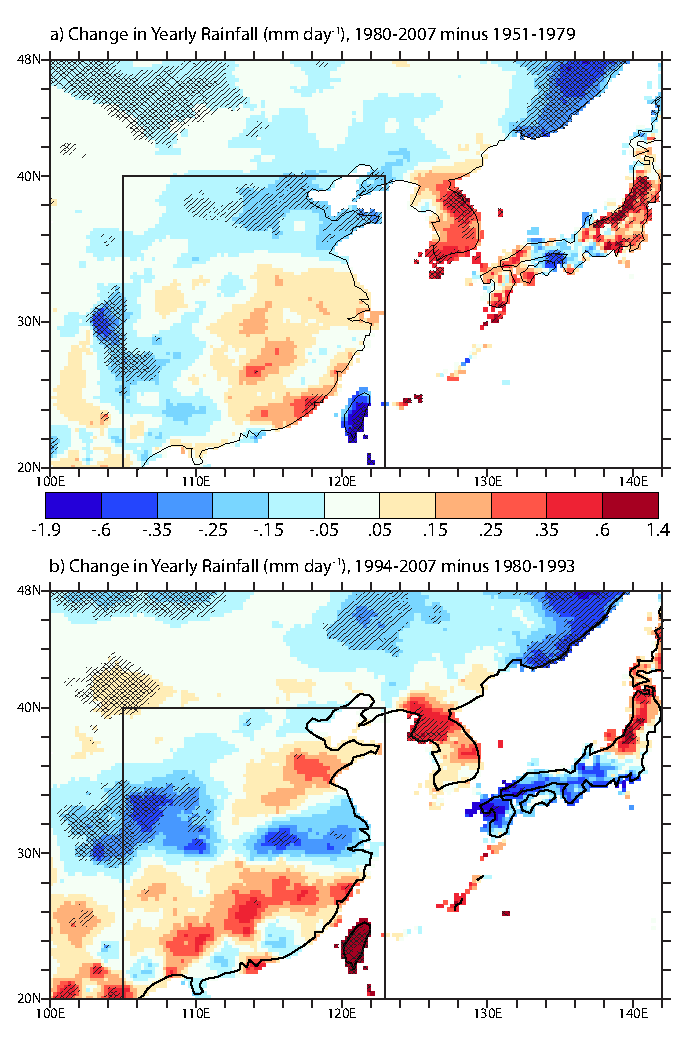
\includegraphics[width=36pc]{Figures/SFND}
\caption{Difference in yearly mean rainfall between 1980-2007 and 1951-1979. The South Flood-North Drought pattern is visible between 110-124$^{\circ}$E and 22-42$^{\circ}$N over mainland China (marked by box). Changes significant at a 95\%/99\% level are marked with single/double cross-hatches respectively.}
\label{fig:f31}
\end{figure}

%%FIGURE 3.8 Changes in Meiyu and rainfall behavior between 1951-1979 and 1980-2007
\begin{figure}[htbp]
\centering
\noindent\includegraphics[width=36pc]{Figures/changes}
\caption{a) 15-day running mean of the change in rainfall between 1951-1979 and 1980-07, with 95\%/99\% confidence level marked by single/double cross-hatches; b) 15-day running mean of the change in rainband frequency between 1951-1979 and 1980-07, with two-degree smoothing in latitude and confidence levels marked as in a). The significance of rainfall changes is calculated by a permutation method. Time periods are marked as in Figure~\ref{fig:hov}: 1 - Spring Rains; 2 - Pre-Meiyu; 3 - Meiyu; 4 - Post-Meiyu; 5 - Fall Rains.}
\label{fig:changes}
\end{figure}


\end{document}